\chapter{First Chapter Title}

Each chapter should begin at the top of a new page, with a two-inch top margin.\footnote{This is your first footnote, if your chosen style manual calls for footnotes rather than endnotes.}
The following text is only included to take up space and provide a visual sense of the layout of your paper.
It is written in Latin for no other reason than to encourage you to bypass it as not being necessary information for you to spend your time reading.
\blindtext[1] \footnote{This is your second footnote. There should be a space, as shown, between each note (whether footnote or endnote).}

\section{First Section Heading}

\blindtext[2]
\endnote{This is your first endnote. It will appear at the end of the document.}

\begin{figure}[ht]
\textit{Follow this list to ensure your pages are in the correct order.}
    \begin{enumerate}
        \item Title page
        \item Copyright notice
        \item Committee page
        \item Abstract
        \item Dedication *
        \item Acknowledgements *
        \item Table of Contents
        \item List of tables \dag
        \item List of figures \dag
        \item List of plates \dag
        \item List of abbreviations \ddag
        \item Body of manuscript
        \item Appendix(es) \ddag
        \item Notes \ddag
        \item Bibliography
    \end{enumerate}
\caption[Sequence of pages for thesis or dissertation]{Sequence of pages for thesis or dissertation. Pages are mandatory unless marked with one of the following symbols. *: Optional. \dag: Include if manuscript uses these. \ddag: Include if necessary.}
\label{fig:sequence-pages}
\end{figure}

\section{Second Section Heading}
\blindtext

\begin{figure}[p]
    \centering
    \rotatebox{90}{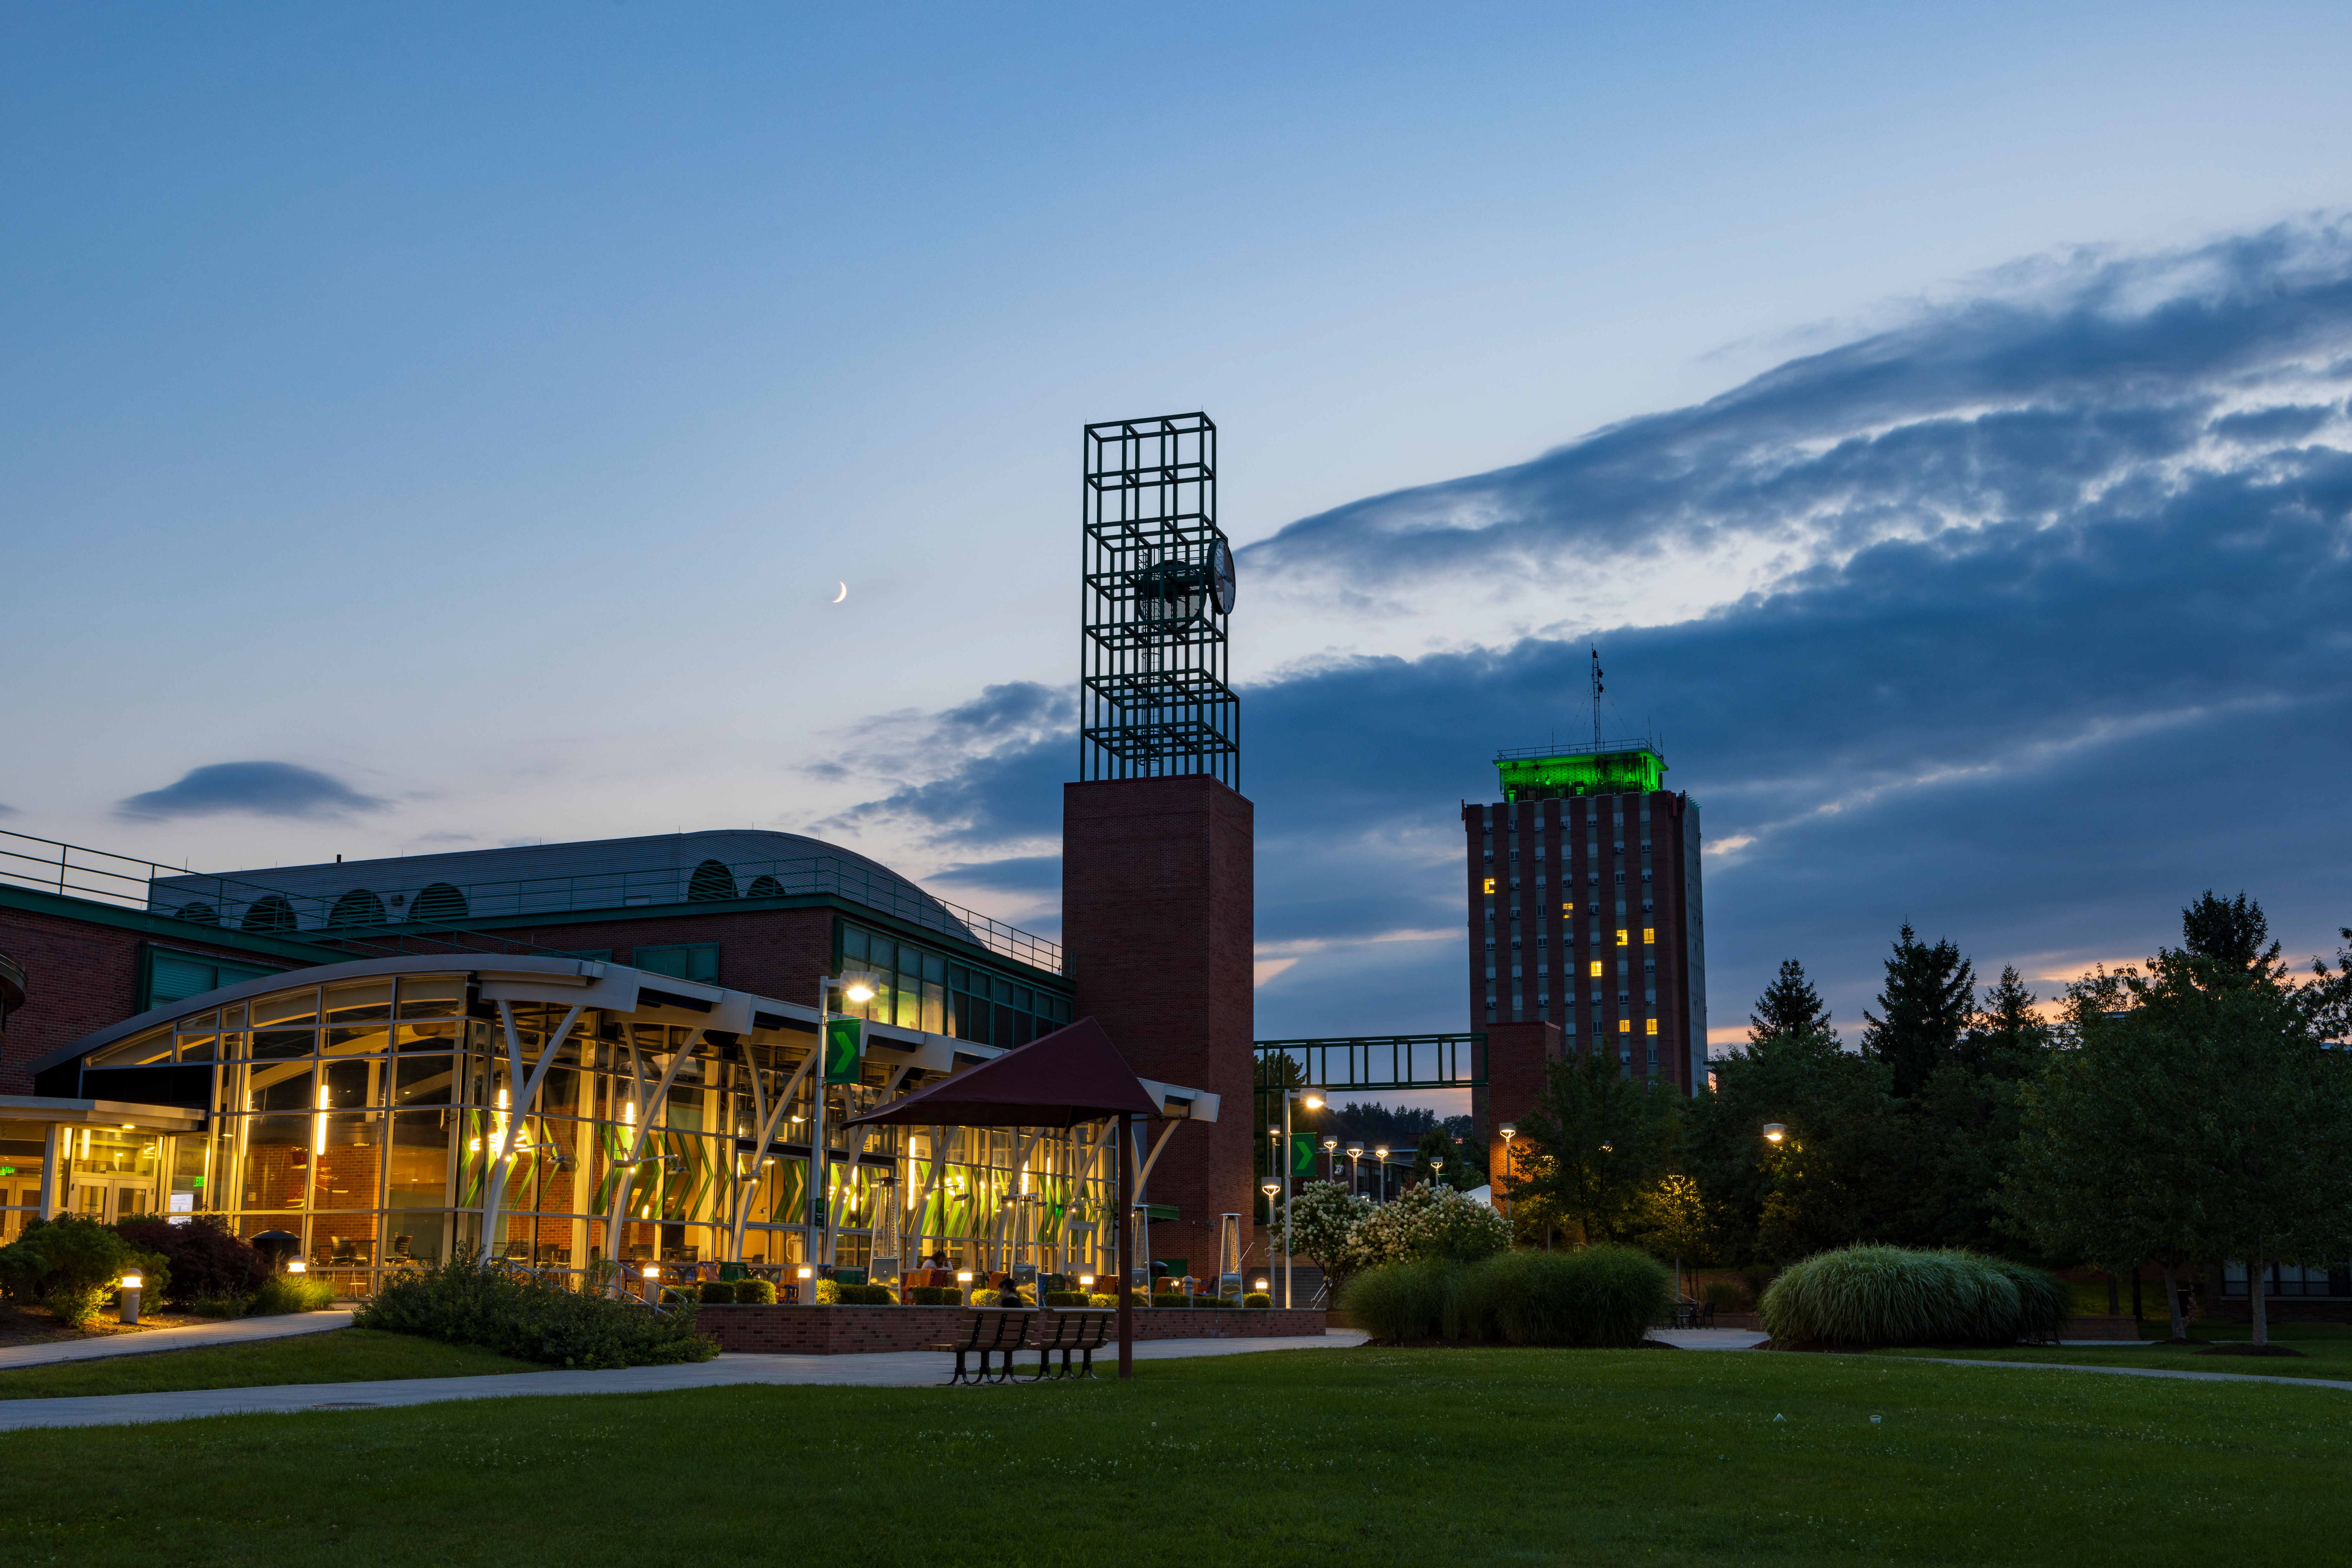
\includegraphics[width=.85\textheight]{photograph.jpg}}
    \caption{The crescent moon sets over the Clock Tower at the Union and the Glenn G. Bartle Library Tower at sunset, August 20, 2023.~\cite{BinghamtonUniversity2023Crescent}}
    \label{fig:photograph}
\end{figure}

\blindtext

\begin{figure}[t]
    \centering
    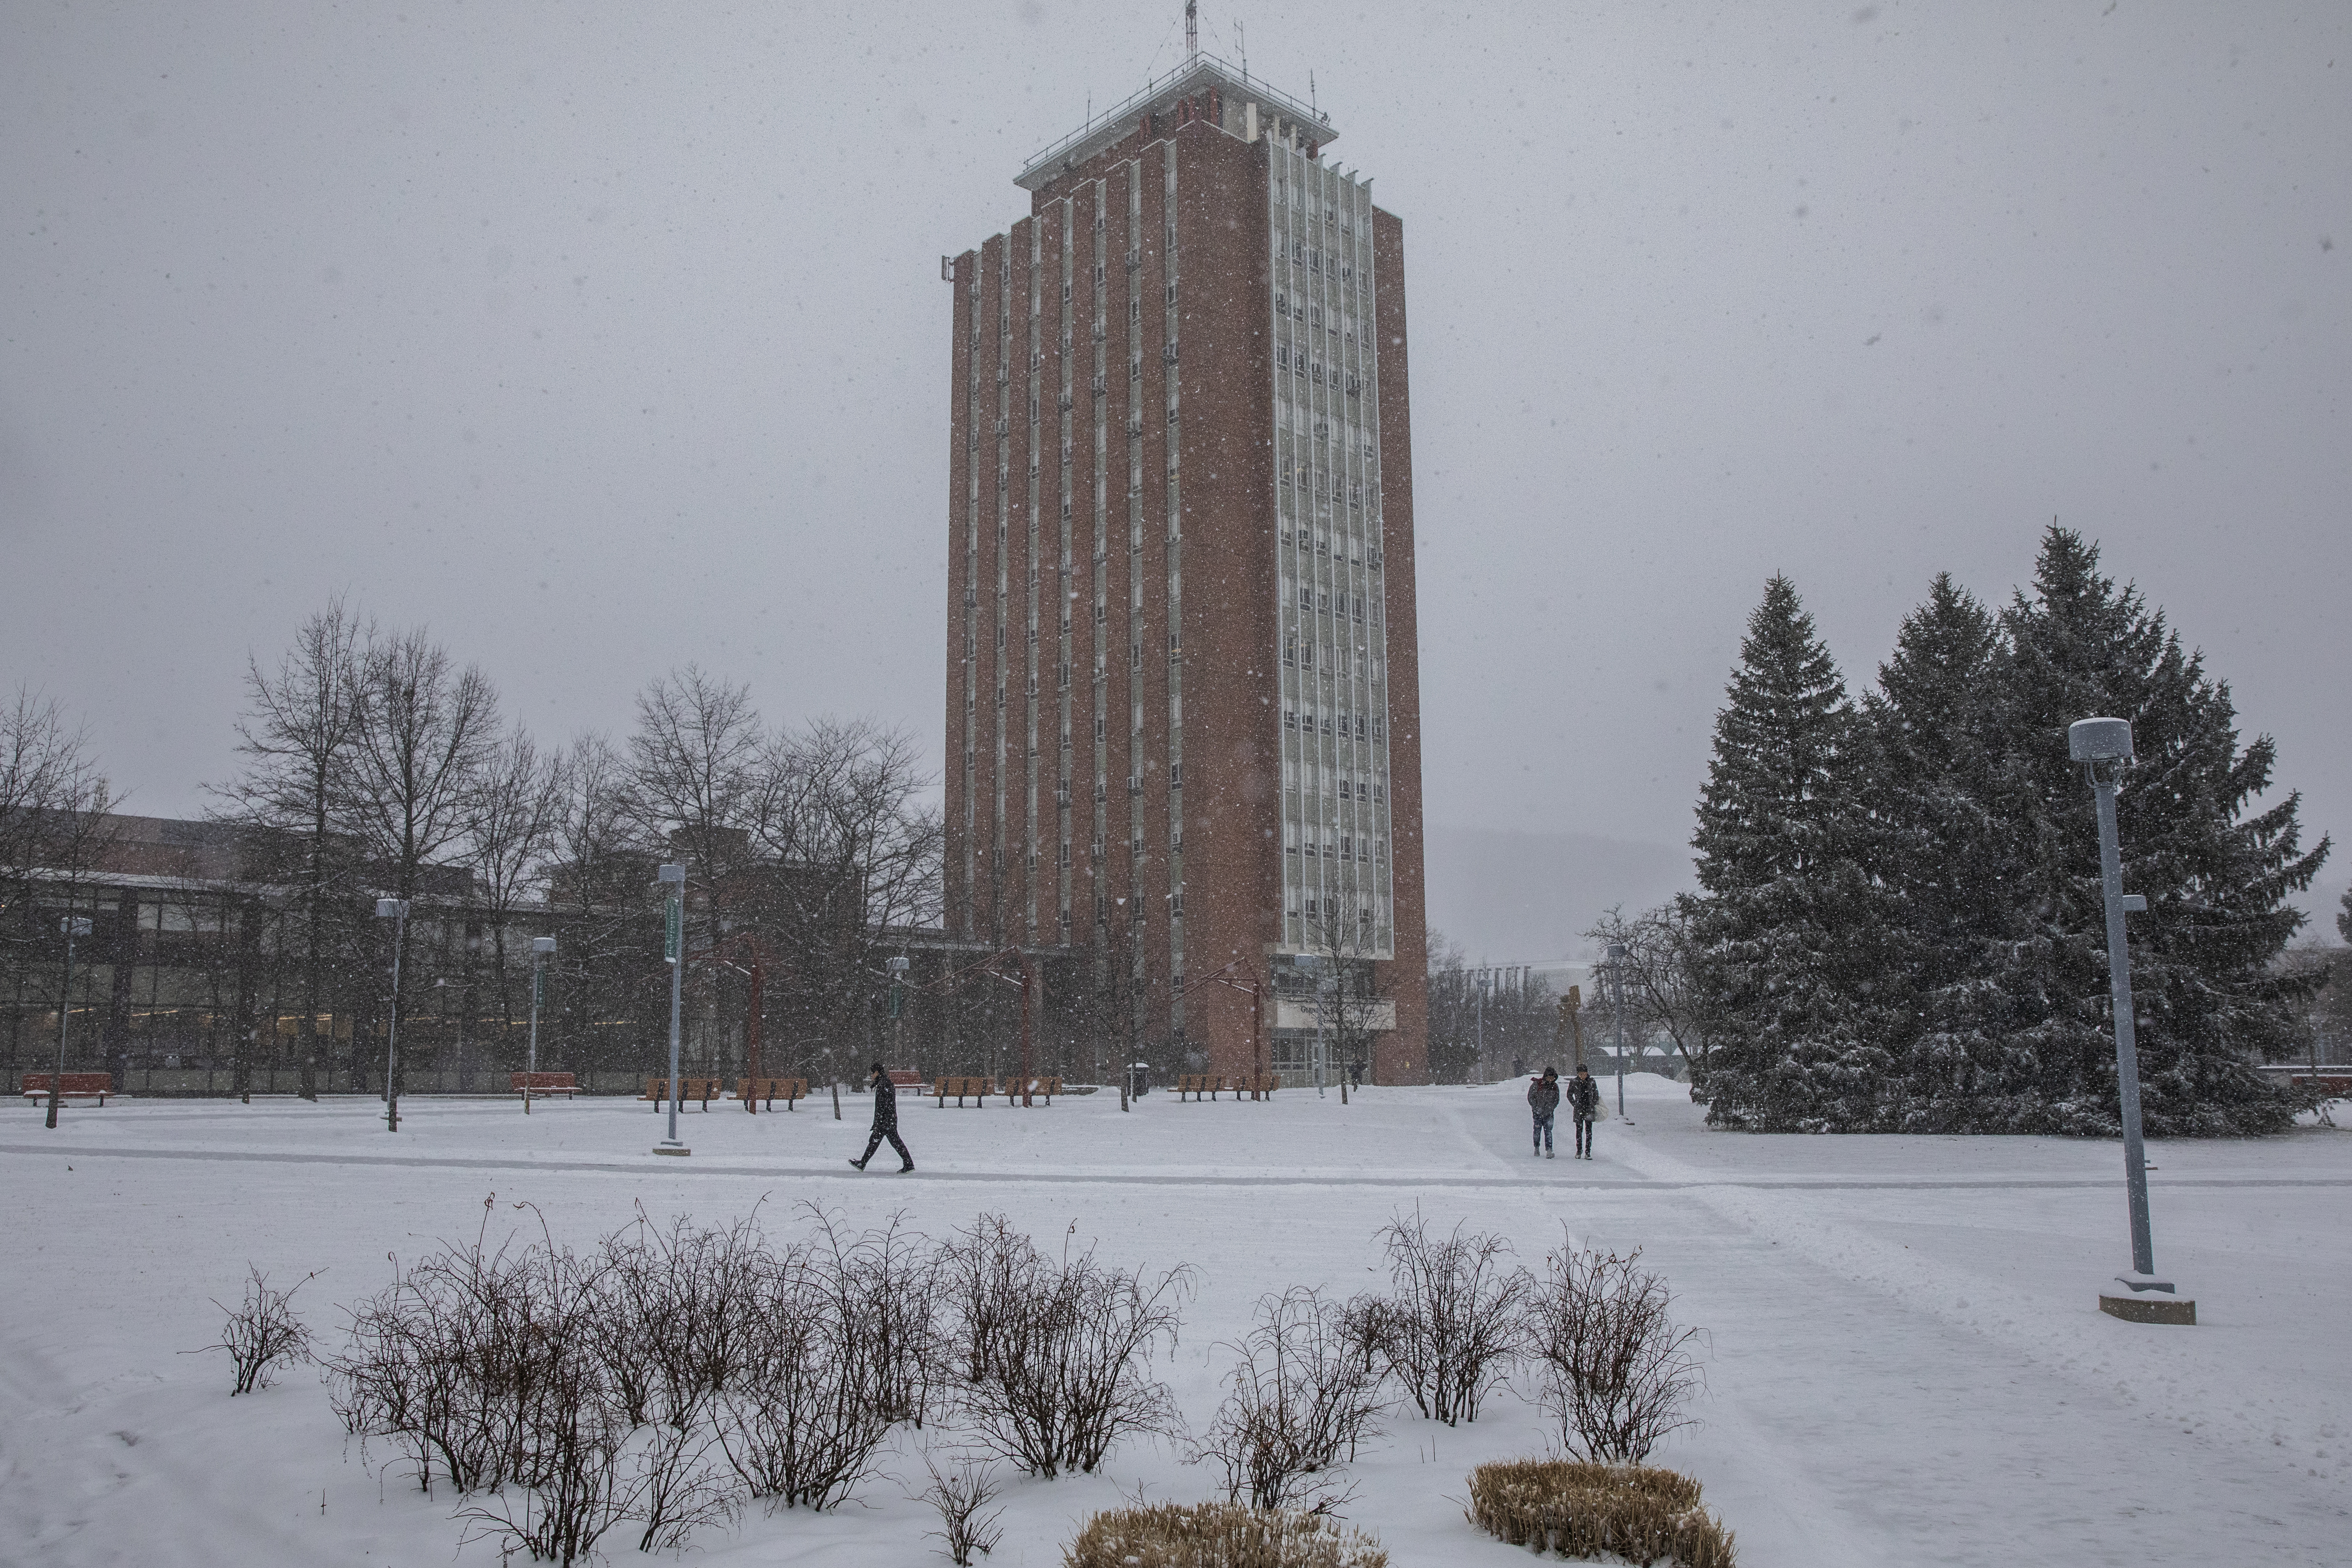
\includegraphics[scale=0.2]{figures/photograph2.jpg}
    \caption{Snowfall at Binghamton University, Tuesday, February 12, 2019. Glenn G. Bartle Library tower.~\cite{BinghamtonUniversity2023Snowfall}}
    \label{fig:photograph2}
\end{figure}

\blindtext

% Please add the following required packages to your document preamble:
% \usepackage{graphicx}
\begin{table}[p]
    \resizebox{\textwidth}{!}{%
    \begin{tabular}{p{5.5cm}|p{10cm}|l}
\hline
\textbf{Formatting Requirement} &
   &
  \textbf{Fulfilled?} \\ \hline
{\textbf{Page margins}} &
  1.5" left margin, 1" all other margins. The 1.5" left margin leaves room for the manuscript to be bound &
   \\ \hline
{\textbf{Body text of manuscript}} &
  Double-spaced. Justifying the text at the right margin is optional &
   \\ \hline
{\textbf{Font size}} &
  No smaller than 10-point and no larger than 14-point &
   \\ \hline
{\textbf{Text color}} &
  All text should be black (including URLs) &
   \\ \hline
{\textbf{New chapter}} &
  Each chapter begins at the top of a new page, with a 2" top margin &
   \\ \hline
{\textbf{Prefatory headings, chapter names, and section headings}} &
  All prefatory headings, chapter names, and section headings should be formatted consistently &
   \\ \hline
{\textbf{Footnotes or endnotes}} &
  Single-spaced, with a double space between each note &
   \\ \hline
{\textbf{Bibliographic entries, works cited, references}} &
  Single-spaced, with an extra space between entries. Style and format should otherwise follow the style guide used for the rest of the thesis/dissertation &
   \\ \hline
{\textbf{Long quotations}} &
  May be indented and single-spaced, though some style guides prefer them to be indented and double-spaced &
   \\ \hline
{\textbf{Tables and figures}} &
  Must conform to the same margins as the text. If the table or figure is placed in landscape orientation (horizontally on page), the margins and page-number location must retain a portrait (vertical) orientation, as on a regular page. Tables and figures may be in color &
   \\ \hline
{\textbf{Table and figure captions}} &
  Single spaced. Should be in the same type as the body of the text &
   \\ \hline
{\textbf{Hand lettering}} &
  Not permitted. Symbols, accent marks, and equations must be typescript &
   \\ \hline
{\textbf{Corrections in pen or pencil}} &
  Not permitted &
   \\ \hline
{\textbf{Printed manuscript}} &
  Single-sided (simplex). Do not staple. Do not hole-punch. The manuscript should be clearly readable throughout, for both electronic and printed documents. Any photocopies should be checked to make sure they are legible. If there are questions regarding print quality, you are encouraged to consult The Graduate School &
   \\ \hline
\end{tabular}%
    }
    \caption{General formatting requirements for thesis or dissertation}
    \label{tab:general-formatting}
\end{table}